\newpage
\section{银河系结构与动力学}

\subsection{银河系的结构}

银河系的恒星分布主要在银盘, 银晕, 与核球. 
\begin{figure}[!htb]
    \centering
    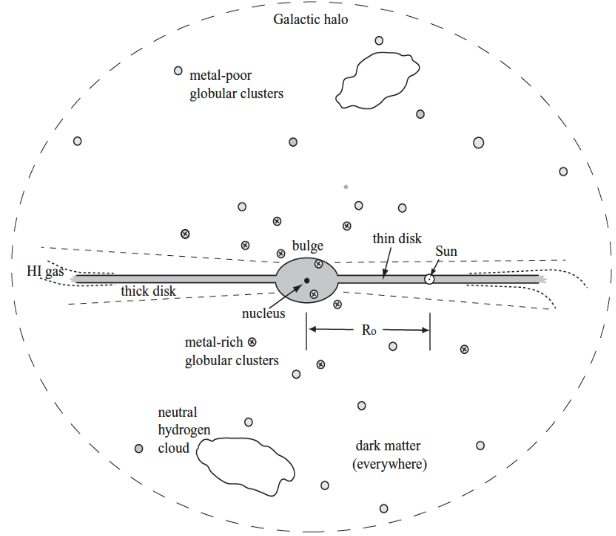
\includegraphics[width=0.42\textwidth]{GA4/银河系的结构}
    \caption{银河系的结构}
\end{figure}

\begin{enumerate}
    \item 银晕 (Galactic halo)
    \begin{itemize}\small
        \item 晕星: 单独存在的恒星, 主要是老年, 贫金属恒星(Pop II). 总质量$\sim 10^9 M_{\odot}$
        \item 球状星团: 几百到上百万颗恒星组成的致密结构
        \item 高速云: 主要是快速运动$(>100 km/s)$的中性氢团块
        \item 气体晕: 温热气体($10^5$-$10^6$K),质量$\sim 10^{11}M_{\odot}$( 非常不确定)
        \item 暗物质晕: 普遍存在于银河系中, 其质量$\sim 10^{12}M_{\odot}$,空间分布$\sim 200 Kpc$
    \end{itemize}
    \item 恒星盘 (disk)
    \small \subitem 银河系的恒星(主要为Pop I)主要分布在一个盘上, 其半径$\sim 15 Kpc$,总质量(5-10)$\times 10^{10} M_{\odot}$太阳在距离银心$\sim 8.5Kpc$的距离处
    \item \normalsize 核球 (Bulge)
    \small \subitem 核球恒星质量$\sim 10^{10} M_{\odot}$
\end{enumerate}

\subsubsection{银晕}
\begin{enumerate}\small
    \item 晕星: 银河系晕中的恒星主要来自银河系的卫星星
    系以及银河系内早期生成的贫金属星. 卫星星系在进入银河系后被潮汐剥离, 剥离出的恒星形成所谓的星流(star stream) . 星流中的恒星一般具有相同的速度和金属丰度. 银河系中最有名星流是人马座星流(Sagittarius Stream). 
    
    \item 星团: 
    \begin{itemize}
        \item 疏散星团
        \begin{itemize}\small
            \item 恒星数目: 从几十到几千不等
            \item 空间尺度: 无规则形状和明显边界, $\sim$ 1-10 pc
            \item 成员星: 存在大量年轻恒星、尘埃和气体
            \item 空间分布: 主要分布在银河系盘上及附近, 银河系有 1000-2000个疏散星团
        \end{itemize}
        \item 球状星团
        \begin{itemize}\small
            \item 恒星数目: 从几千到几百万
            \item 空间尺度: 具有明显的球状和边界, 10$\sim$100 pc, 恒星密度非常高, 平均距离0.1光年
            \item 成员星: 成员星具有同样年龄>100亿、贫金属
            \item 空间分布: 主要在银晕, 目前银河系已经发现$\sim$200个(相比之下M87有15,000个球状星团)
        \end{itemize}
    \end{itemize}
\end{enumerate}

\subsubsection{银盘}
\begin{enumerate}\small
    \item 薄盘: 大部分恒星分布在薄盘, 占盘恒星总数90\% 以上. 一般假设盘上的恒星分布为轴对称, 其径向和垂直方向分布为指数盘
    \begin{align*}
        n\sim \frac{n_0}{2Z_0}e^{-\frac{r}{Rs}\frac{|z|}{Z_0}}
    \end{align*}
    $Rs$为特征半径$\sim$3.5 Kpc, $Z_0$ 为特征标高$\sim$0.2Kpc. 
    \item 厚盘: 占盘上恒星总数10\%, 其恒星分布类似薄盘, 特征标高$\sim$1 Kpc. 厚盘上的恒星年龄老, 金属丰度低
\end{enumerate}

银河系盘具有旋转, 盘上的恒星围绕银河系中心旋转, (太阳的旋转速度$\sim$200km/s), 但是也存在一定的本动速度($\sim$10-20km/s)一般认为厚盘上的恒星来自早期薄盘上形成的恒星, 在径向迁移过程中形成的. 

\subsubsection{银河系中心与核球}
\begin{enumerate}\small
    \item 核球: 银河系中心是一个核球, 其中恒星年龄老, 其
    密度分布一般认为满足如下形式(Hernquist Profile)
    \begin{align*}
        \rho \sim \frac{a}{r\times(r+a)^3}
    \end{align*}
    $a$为特征半径$\sim$0.6 Kpc
    \item 银河系中心: 位于人马座方向(Sagittarius), 一致认为
    其中心物体可能是一个黑洞, 命名为SgrA*. 确定其中心天体的质量$\sim$400万太阳质量. 
\end{enumerate}

\subsubsection{暗物质}
研究表明银河系含有大量暗物质, 其质量和空间分布远远超过其恒星分布. 测量银河系的暗物质分布是目前研究的前沿, 但是对于其质量测量还存在巨大争议, 但是整体质量集中在$8\times 10^{11} M_{\odot}$ 到$2\times 10^{12} M_{\odot}$之间, 暗物质的空间分布大约为200-250 kpc. 

\subsubsection{盘星系}

\begin{figure}[!htb]
    \centering
    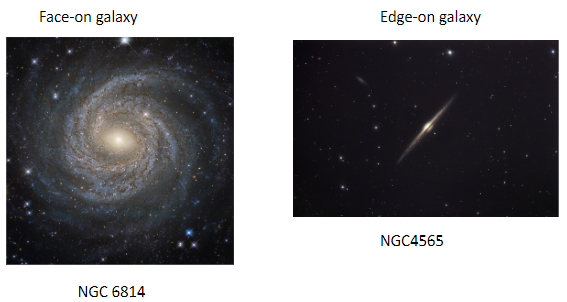
\includegraphics[width=0.42\textwidth]{GA4/盘星系}
    \caption{盘星系}
\end{figure}

对于盘状星系, 如果沿着垂直盘方向观测, 称为正向(Face on), 沿着侧面观测, 称为edge on. 实际上我们并没有选择观测方向的自由, 但是宇宙中的大量星系给我们提供了不同正向星系和侧向星系的样本. 

Face-on Galaxy
\begin{itemize}\small
    \item 优势
    \subitem 很容易辨认是否是盘星系
    \subitem 能够分辨出核球和盘, 以及看到明显的旋臂
    \item 缺点
    \subitem 无法测量其旋转速度
    \subitem 很难搜寻其卫星星系(被前景恒星遮挡)
\end{itemize}

Edge-on Galaxy
\begin{itemize}\small
    \item 优势: 可以测量其旋转曲线, 寻找卫星星系等
    \item 缺点: 很难鉴别其是否是盘主导的星系, 特别是在中等倾角的情况下
\end{itemize}

\subsubsection{银河系的旋臂}
银河系是典型的盘星系, 其包含4个明显的旋臂: 英仙臂(Perseus Arm), 人马旋臂(Sagitarrius arm), 矩尺-天鹅臂(Norma-Cygnus arm), 盾牌-南十字臂(Scutum-Crux arm). 太阳位于猎户座旋臂(Orion Spur). 旋臂是恒星、气体密集聚集的区域. 旋臂并不是固定的物质臂, 而是一种密度波. 

\subsubsection{较差自转 (differential rotation)}
指天体的不同部位存在不同的角速度. 对于刚体(地球表面可近似为刚体), 其不同纬度的角速度相同. 对于只存在引力的系统, 如星系、恒星, 一般存在较差自转现象. 

银河系: 不同位置存在较差自转. 如图所示, 不同半径处的恒星具有较差自转, 内部恒星角速度快, 则经过一个较短时间后将形成旋臂. 随着时间推移, 旋臂将缠绕紧密, 最终缠绕在一起. 但观测则表明盘星系的旋臂并没有缠绕在一起, 于是林家翘等提出了密度波理论, 解释了银河系旋臂问题. 

\begin{figure}[!htb]
    \centering
    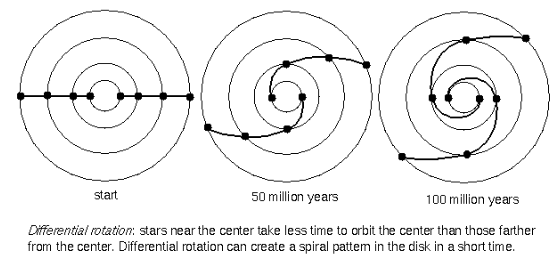
\includegraphics[width=0.42\textwidth]{GA4/银河系较差自转}
    \caption{银河系较差自转}
\end{figure}


\subsubsection{银河系自转}
1927年奥尔特首先考虑到利用恒星的自行和径向速度来测量银河系的旋转. 他假设恒星盘都围绕银河系做圆周运动, 如下图所示(这里只考虑盘内运动). 

\begin{figure}[!htb]
    \centering
    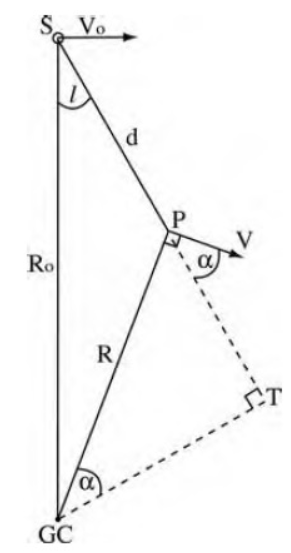
\includegraphics[width=0.159\textwidth]{GA4/恒星的自行和径向速度}
    \caption{恒星的自行和径向速度}
\end{figure}

太阳在$S$处, 沿着银经$l$方向, 距离$d$处测量一个恒星$P$的运动, 在太阳处观测者测量的其径向速度与切向速度分别为
\begin{align*}
    V_r&=V\cos\alpha-V_0\sin l\\
    V_t&=V\sin\alpha-V_0\cos l
\end{align*}
利用三角函数关系$\frac{\sin l}{R}=\frac{\sin(90^{\circ}-\alpha)}{R_0}$可得
\begin{align*}
    V_r=\left( \frac{V}{R}-\frac{V_0}{R_0} \right)R_0\sin l
\end{align*}
为了将其表达为$(d, l)$的函数, 在观测者太阳处将$\frac{V}{R}$对$R$泰勒展开到二阶
\begin{align*}
    \frac{V}{R}&\approx \frac{V_0}{R_0}+ \left.\frac{d\frac{V}{R}}{R}\right|_{R_0} (R-R_0) \\
    &=\frac{V_0}{R_0}+\left( \frac{R_0\frac{dV}{dR}- V_0}{R_0^2} \right)(R-R_0)  \\
    &=\frac{V_0}{R_0}+\left( \frac{1}{R_0}\frac{dV}{dR}-\frac{V_0}{R_0^2} \right)(R-R_0)
\end{align*}
在$d$很小时有 $R_0-R=d\cos l$代入可得
\begin{align*}
    V_r\approx-\frac{1}{2} \left(\frac{dV}{dR}-\frac{V_0}{R_0} \right)d\sin 2l
\end{align*}
定义奥尔特常数$\displaystyle A=-\frac{1}{2} \left(\frac{dV}{dR}-\frac{V_0}{R_0} \right)$, 可得
\begin{align*}
    V_r=Ad\sin 2l
\end{align*}

对于切向速度, 利用 $R_0\cos l=R\sin \alpha +d$可得
\begin{align*}
    V_t=&\left( \frac{V}{R}-\frac{V_0}{R_0} \right) R_0\cos l-V\frac{d}{R}\\
    =&- \left(\frac{dV}{dR}-\frac{V_0}{R_0} \right)d\cos^2 l - \frac{V}{R}d\\
    =&-\frac{1}{2} \left(\frac{dV}{dR}-\frac{V_0}{R_0} \right)d\cos 2l -\left(\frac{1}{2} \left(\frac{dV}{dR}-\frac{V_0}{R_0} \right)+ \frac{V}{R}\right) d\\
    \approx &-\frac{1}{2} \left(\frac{dV}{dR}-\frac{V_0}{R_0} \right)d\cos 2l-\frac{1}{2} \left(\frac{dV}{dR}+\frac{V_0}{R_0} \right)d
\end{align*}
同理定义奥尔特常数$\displaystyle B=-\frac{1}{2} \left(\frac{dV}{dR}+\frac{V_0}{R_0} \right) $, 可得
\begin{align*}
    V_t\approx Ad\cos2l+Bd
\end{align*}

\begin{figure}[!htb]
    \centering
    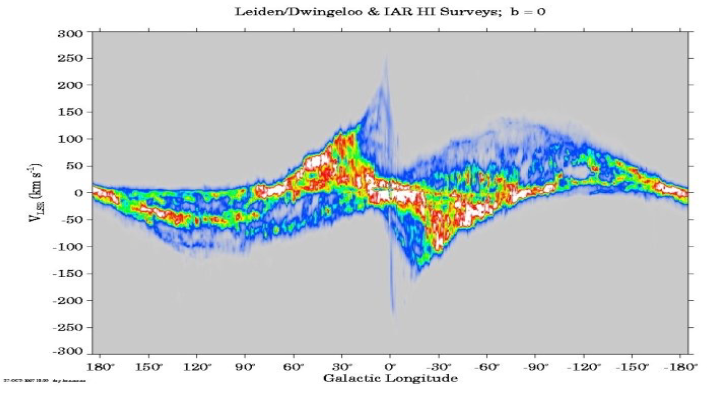
\includegraphics[width=0.479\textwidth]{GA4/旋转曲线}
    \caption{利用21cm观测到银河系内中性氢的旋转曲线 (相对于太阳)}
\end{figure}

利用依巴谷卫星测量的恒星自行和视向速度等数据, 得到了银河系一些局部参数. 
\begin{table}[!htb]
    \centering
    \caption{银河系一些局部参数}
    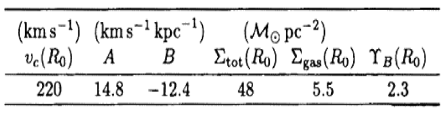
\includegraphics[width=0.309\textwidth]{GA4/银河系一些局部参数}
\end{table}

利用$A-B=\frac{V_0}{R_0}$与$R_0\approx 8$Kpc, 可知$V_0\approx 220$km/s. 由此可知, 太阳围绕银河系中心一圈需要2.2亿年, 目前已经绕银心运动了$\sim$20圈. 

直接的测量太阳旋转的速度是测量银河系中心SgrA${}^*$的自行. 利用VLA对该源的自行测量数据为 
\begin{align*}
    (u_l,u_b)=(-6.55, -0.48) \text{mas/yr}
\end{align*} 
由此得到太阳的旋转速度为$\sim$240km/s. 与利用奥尔特常数得到的结果比较接近. 

\subsubsection{银河系的旋转曲线}
对于漩涡星系, 其质量可以通过测量示踪天体的旋转速度来得到. 由牛顿定律可知, 
旋转速度取决于某个半径内的总质量
\begin{align*}
    V(r)=\sqrt{\frac{GM(<r)}{r}}
\end{align*}
$M(<r)$是半径 $r$ 以内包含的总质量. 

而星系的物质主要由恒星, 气体和暗物质构成
\begin{align*}
    M(r)=M_{disk}(r)+M_{bulge}(r)+M_{gas}(r)+M_{dm}(r)
\end{align*}
恒星和气体的分布可以通过观测直接得到, 再利用最佳拟合旋转曲线, 并得到暗物质的分布和总质量. 

对银河系, 一般采取下面的模型来描述物质分布
\begin{enumerate}
    \item 指数盘
    \begin{align*}
        \rho_d (r,\ z)=\frac{\Sigma_0}{2 z_d}\exp\left( -\frac{|z|}{z_d}-\frac{r}{R_d} \right)
    \end{align*}
    盘质量$M_{disk}=2\pi \Sigma_0 R_d^2=5\times 10^{10}M_{\odot},\ R_d=3.6\text{kpc},\ z_d=0.3\text{kpc}$
    \item 核球
    \begin{align*}
        \rho \sim \frac{a}{r(r+a)^3}
    \end{align*}
    特征半径 $a\sim 0.6\text{Kpc},\ M_{bulge}=9\times 10^9 M_{\odot}$
    \item 暗物质晕
    \begin{align*}
        \rho_{dm}=\frac{\rho_c}{x^{r}(1+x)^{3-\gamma}}
    \end{align*}
    $x=\frac{r}{R_h}$, $R_h$为特征半径. 对于NFW暗晕密度分布, $\gamma =1$. 
\end{enumerate}

测量旋转曲线的方法只适用于银盘, 且通常只能到20 Kpc左右. 旋转曲线可以很好的用几个物质分量来拟合: 中央黑洞、内核球、主核球、盘、暗物质. 
\begin{itemize}\small
    \item 从银心到太阳处, 银盘上恒星的引力势占主导. 
    \item 在$\sim$30Kpc以外, 示踪天体来自银晕, 这些天体并非开普勒运动, 因此无法利用旋转速度来得到暗晕质量. 
\end{itemize}

\subsection{星系动力学}

\subsubsection{基础}
\begin{figure}[!htb]
    \centering
    \begin{tikzpicture}
        \draw (0, 0) [fill=light_blue] circle (1.2);

        \draw [thick, ->, draw=light_red] (0:1.2)--(0, 0)--(60: 1.2) node [above right] {$\vec{e_\theta}$};
        \draw [dashed, ->, draw=white] (0, 0)--(70:1.2) node [midway, left] {$r\vec{e_r}$};

        \path (60:0.6)--(0:0.6) node [midway] {$\theta$};

        \draw (65:0.6)--(30:1.5) node [right] {$d\theta$};
    \end{tikzpicture}
\end{figure}

恒星在球对称引力势中的运动, 其位矢$\vec{r}=r\vec{e_r}$, 运动可表示为
\begin{align*}
    \ddot{r}=F(r)\vec{e_r}
\end{align*}
在极坐标下对$\vec{r}$求导, 结合$d\vec{e_r}=d\theta\vec{e_\theta},\ d\vec{e_\theta}=-d\theta\vec{e_r}$, 有
\begin{align*}
    \frac{d\vec{r}}{dt}=\frac{d(r\vec{e_r})}{dt}=\dot{r}\vec{e_r}+r\frac{d\vec{e_r}}{dt}=\dot{r}\vec{e_r}+r\dot{\theta}\vec{e_\theta}
\end{align*}
在此求导得
\begin{align*}
    \ddot{r}=(\ddot{r}-r\dot{\theta}^2)\vec{e_r}+(2\dot{r}\dot{\theta}+r\ddot{\theta})\vec{e_\theta}=F(r)\vec{e_r}
\end{align*}
因此有
\begin{align}
    \ddot{r}-r\dot{\theta}^2&=F(r) \label{C1} \\ 
    2\dot{r}\dot{\theta}+r\ddot{\theta}&=0 \label{C2}
\end{align}

由(\ref{C2})可得$\displaystyle \frac{d(r^2\dot{\theta})}{dt}=0$, 即$r^2\dot{\theta}=L$ (常数, 角动量). 将$\theta$来替代$t$作为自变量, 即有
\begin{align*}
    \frac{dy}{dt}=\frac{L}{r^2}\frac{dy}{d\theta}
\end{align*}

(\ref{C1})可变为
\begin{align*}
    \frac{L^2}{r^2}\frac{d\left( \frac{1}{r^2}\frac{dr}{d\theta} \right)}{d\theta}-\frac{L^2}{r^3}=F(r)
\end{align*}
令$\mu=\frac{1}{r}$, 可得
\begin{align}
    \frac{d^2\mu}{d\theta^2}+\mu =-\frac{F(\frac{1}{\mu})}{L^2\mu^2} \label{C3}
\end{align}
该方程可以数值求解, 在特殊情况下有解析解. 

对(\ref{C3})两边同乘$\frac{d\mu}{d\theta}$并对$d\theta$积分, 利用$F=-\nabla \phi$可得
\begin{align*}
    \left( \frac{d\mu}{d\theta} \right)^2+2\frac{\phi}{L^2}+\mu^2=Constant
\end{align*}
令$Constant=2\frac{E}{L^2}$, 则有
\begin{align}
    E=\frac{1}{2}\left( \frac{dr}{dt} \right)^2+\frac{1}{2}\left( r\frac{d\theta}{dt} \right)^2+\phi(r) \label{C4}
\end{align}
显然该常数就是单位质量的总能量. 

对于束缚轨道, 一定$\exists \mu$, 有$\frac{d\mu}{d\theta}=0$, 此时$\mu$满足
\begin{align*}
    2\frac{\phi(\frac{1}{\mu})}{L^2}+\mu^2=2\frac{E}{L^2}
\end{align*}
可解得$\mu_1, \mu_2$, 因此恒星径向位置将在$\mu_1, \mu_2$之间振荡. 

(\ref{C4})可写为
\begin{align*}
    \frac{dr}{dt}=\pm\sqrt{2(E-\phi)-\frac{L^2}{r^2}}
\end{align*}
在近心点与远心点处有$\frac{dt}{dt}=0$. 径向周期为
\begin{align*}
    T_r=2\int_{r_1}^{r_2}\frac{dr}{\sqrt{2(E-\phi)-\frac{L^2}{r^2}}}
\end{align*}
同时从近心点到远心点再到近心点, 方向角$\theta$的变化量为
\begin{align*}
    \Delta \theta&=2\int_{r_1}^{r_2}\frac{d\theta}{dr}dr=2\int_{r_1}^{r_2}\frac{L}{r^2}\frac{dt}{dr}dr\\
    &=2L\int_{r_1}^{r_2}\frac{dr}{r^2\sqrt{2(E-\phi)-\frac{L^2}{r^2}}}
\end{align*}

在$T_r$时间内, 恒星角向位置的变化率为$\Delta \theta$, 意味着恒星角速度为$\omega=\frac{\Delta\theta}{T_r}$, 因此其角向周期$T_\theta=\frac{2\pi}{\omega}=\frac{2\pi}{\Delta \theta}T_r$. 一般来说, $\frac{2\pi}{\Delta\theta}$不可能是有理数, 因此轨道不会是闭合的, 即恒星角位置变化$2\pi$以后, 恒星的径向位置并未回到原来的值. 

在大部分情况下, 在球对称引力势中恒星的典型轨道为玫瑰花节. 

\begin{figure}[!htb]
    \centering
    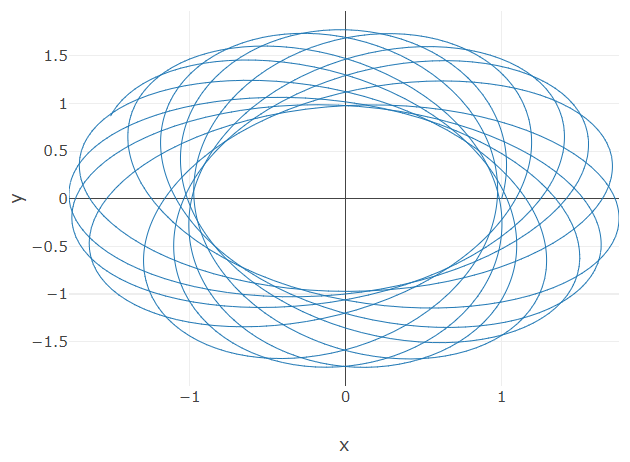
\includegraphics[width=0.309\textwidth]{GA4/恒星的典型轨道}
    \caption{恒星的典型轨道}
\end{figure}

在某些特殊情况下, 轨道是闭合的
\begin{enumerate}
    \item 均匀球产生的引力势
    \begin{align*}
        x&=X\cos (\Omega t+\epsilon_x)\\
        y&=Y\cos (\Omega t+\epsilon_y)
    \end{align*}
    \item 点质量产生的引力势(开普勒运动)
    \begin{align*}
        \mu(\theta)=C\cos(\theta-\theta_0)+\frac{GM}{L^2}
    \end{align*}
\end{enumerate}


\subsubsection{潮汐半径 (tidal radius)}
观测发现处于银河系晕中的球状星团 (或者处于星系团中的单个星系) 都有非常明显的边界. 这一效应叫潮汐剥离 (tidal stripping). 
\begin{figure}[!htb]
    \centering
    \begin{tikzpicture}
        \coordinate (C1) at (-3.2, -3.2);
        \coordinate (C2) at ( 0,  0);
        \draw[fill=light_blue] (C1) circle (0.64);
        \node [below= 0.7 of C1] {$M$};
        \draw[fill=light_blue] (C2) circle (0.5);
        \node [below= 0.6 of C2] {$m, r$};

        \draw [draw=light_red] (C1)--(C2) node [midway, left] {$D$};
        \draw [draw=white] (C2)--(120:0.5) node [above] {$p$};
    \end{tikzpicture}
    \caption{潮汐半径}
\end{figure}

系统$m$在系统$M(>m)$的引力场中运动, $m$点中心受到$M$的引力, $m$点表面半径$r$处一点$p$受到$M$的引力, 与$p$还受到$m$点的引力分别为
\begin{align*}
    F_{mM}=\frac{GM}{D^2},\ F_{pM}=\frac{GM}{(D-r)^2},\ F_{pm}=\frac{Gm}{r^2}
\end{align*}
$D$为 $(M, m)$的质心距离. 

如果$p$的加速度大于$m$中心点的加速度, 则$p$与$m$中心的距离将变大, 导致$m$的物质损失, 该现象为潮汐剥离. 

由
\begin{align*}
    \frac{GM}{(D-r)^2}-\frac{Gm}{r^2}&>\frac{GM}{D^2}\\
    \frac{GM}{(D-r)^2}-\frac{GM}{D^2}&>\frac{Gm}{r^2}\\
\end{align*}
在$D\gg r$的情况下, 有
\begin{align*}
    2GM\frac{r}{D^3}>\frac{Gm}{r^2}
\end{align*}
得
\begin{align*}
    r>\left( \frac{m}{2M} \right)^{\frac{1}{3}}D
\end{align*}
因此物体$m$在$M$作用下的潮汐半径为
\begin{align*}
    r_t=\left( \frac{m}{2M} \right)^{\frac{1}{3}}D
\end{align*}
该半径之外的物体将被逐渐剥离而损失. 

如果换一种表达方式, 假设卫星星系的平均密度为$\rho_s$, 主星系密度为$\rho$, 半径为$R$, 则可以得到一个临界半径$r$, 一旦卫星星系离主星系的距离$r$满足
\begin{align*}
    r_{lim}<2^{\frac{1}{3}}\left( \frac{\rho}{\rho_s} \right)^{\frac{1}{3}}R
\end{align*}
则卫星星系将被瓦解. Edouard Roche首先得到了该公式, 这个最小距离也称为\textcolor{light_red}{洛希极限}. 

\begin{figure}[!htb]
    \centering
    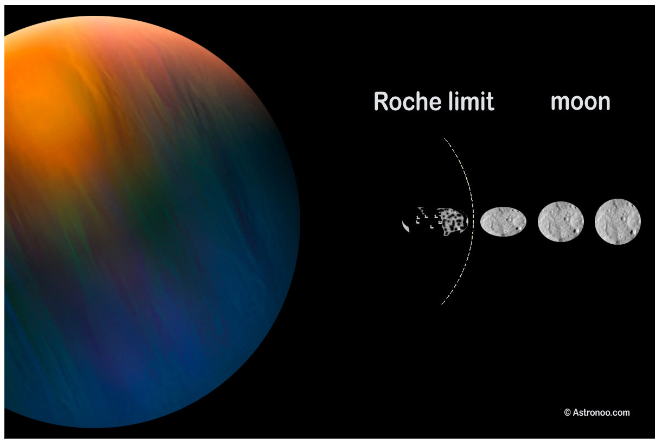
\includegraphics[width=0.309\textwidth]{GA4/洛希极限}
    \caption{洛希极限}
\end{figure}

\subsubsection{动力学摩擦 (Dynamical friction)}
动力学摩擦是一个天体在另一个由背景物质构成的体系中运动时, 由于其受到背景物质的引力, 其运动速度变小(类似于受到摩擦)的现象. 

考虑一个质点M在由背景物质组成的系统中穿越的情况. 由于背景中的每一个物体(黑点)和M之间存在引力, 因此在与M前进方向垂直的方向上, 质点m将受到M的引力, 导致其向M方向运动(图中由上到下/由下到上运动). 一般来说M对m的引力较小, M穿行速度较快, 因此会在M的背后(与前进方向相反)聚集较多的背景粒子, 导致M整体感受到背后聚集物体的引力, 导致其速度V变慢. 该现象为动力学摩擦. 

\begin{figure}[!htb]
    \centering
    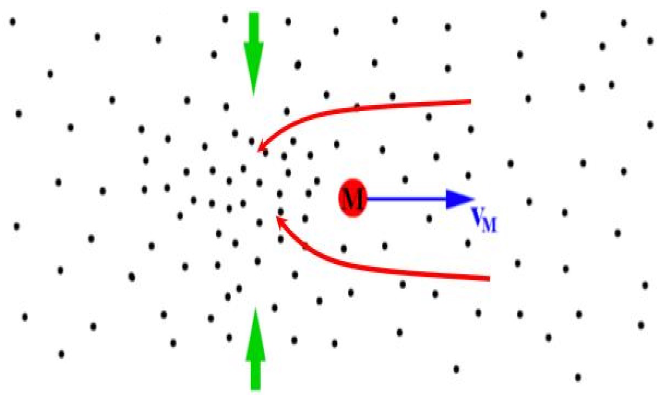
\includegraphics[width=0.309\textwidth]{GA4/动力学摩擦}
    \caption{动力学摩擦}
\end{figure}

动力学摩擦普遍存在: 银河系卫星星系在银河系中运动, 星系在星系团中都会受到动力学摩擦. 由于其速度变慢, 最终导致卫星星系向星系中心靠拢. 

常用的动力学摩擦时标(Dynamical friction time scale). 卫星星系M将在该时标以后损失所有角动量而到达星系中心(质量越小, 时标越长).

\paragraph{两体碰撞的简单示例}
设想质点$m$, 以高速$V$从无穷远( $t=0$时, $x= \infty$) 经过一物体$M$(质量$M$), 由于$M$的引力, 质点$m$将获得一个与原速度$V$垂直 方向的速度$dV_\perp$ ,  如果$dV_\perp$相比$V$很小, 可以得到其偏转角
\begin{align*}
    \alpha \cong \frac{GM}{bV^2}
\end{align*}

\begin{figure}[!htb]
    \centering
    \begin{tikzpicture}
        \coordinate (M) at (0, -1.2);
        \coordinate (m) at (-2.4, 0);

        \draw [draw=light_blue, ->] (-3.2, 0)--(0, 0);
        \draw [draw=light_blue, dashed] (2, 0)--(0, 0);

        \path (m)--(0, 0) node [midway, below] {$x$};
        \draw (0, 0)--(M) node [midway, left] {$b$};

        \draw [fill= light_blue] (M) circle (0.15) node [right] {$M$};
        \draw [fill= light_blue] (m) circle (0.1) node [above] {$m, V$};

        \draw [draw=light_red, dashed, ->] (m)--(M); 
        \draw [draw=light_green, ->] (0, 0)--(-20: 2.4) node [below] {$V$};
        \draw [draw=light_blue, ->] ($(0,0)!(-20:2)!(2,0)$)--(-20:2) node [midway, right] {$dV_\perp$};
    \end{tikzpicture}
    \caption{两体碰撞示例}
\end{figure}

如果$dV_\perp$ 很小, 可以近似认为粒子$m$的路线为直线(蓝色实线+蓝色虚线), 可以得到由于$M$的引力导致在垂直方向获得的速度
\begin{align*}
    dV_\perp&= 2\int F_\perp dt \\
    &=2 \int_0^\infty \frac{GM}{(x^2+b^2)}\frac{b}{\sqrt{(x^2+b^2)}}\frac{dx}{V}\\
    &=2\frac{GM}{V}\int_0^\infty\frac{b}{(x^2+b^2)^{\frac{3}{2}}}dx
\end{align*}
令$x=b\tan \theta$可得
\begin{align*}
    dV_\perp=\frac{2GM}{bV}
\end{align*}
偏转角
\begin{align*}
    \alpha \approx \frac{dV_\perp}{V}=\frac{2GM}{bV^2}
\end{align*}

如果$m$从无穷远过来并逃逸, 速度$V$值不变, 相当于在平行于$V$方向获得一个减速
\begin{align*}
    \Delta V_{\parallel }=V-V\cos\alpha=2V\sin\frac{\alpha^2}{2}\approx 2V\frac{G^2M^2}{b^2V^4}
\end{align*}
该碰撞的结果是粒子$m$获得一个在垂直运动方向的速度$dV_\perp$ (指向$M$),并沿着运动方向的减速$dV_\parallel$, 相当于经历了一个动力学摩擦. 

\subsubsection{潮汐加热}

\begin{figure}[!htb]
    \centering
    \begin{tikzpicture}
        \coordinate (C1) at (0, 0);
        \coordinate (C2) at (-1.6, -2.4);
        \draw [->] (-2.8, -2.4)--(2, -2.4) node [midway, below right] {$V$};

        \draw  [fill=light_blue] (C1) circle (0.64);
        \node [right=0.7 of C1] {$S$};
        \draw [fill=light_blue] (C2) circle (0.5);
        \node [below=0.6 of C2] {$P, M$};

        \draw [draw=light_red] (C1)--(120:0.64) node [midway, right] {$r$} node [above left] {$q$};
        \draw [draw=light_red] (C1)--(C2) node [midway, right] {$R_0$};
        \draw [draw=light_red] (C2)--(120:0.64) node [midway, left] {$R$};
    \end{tikzpicture}
    \caption{潮汐加热}
\end{figure}

如图一个物体$P$(质量$M$), 快速经过一个物体$S$, 考虑$P$对$S$内质点$q$的动力学影响. $q$点位置 $R=R_0+r$, 其运动为$P, S$的引力势叠加
\begin{align*}
    \ddot{R}&=-\nabla_R\phi_P-\nabla_r\phi_S\\
    \ddot{R_0}+\ddot{r}&=-\nabla_R\phi_P-\nabla_r\phi_S
\end{align*}
即有
\begin{align*}
    \ddot{r}&=-\nabla_R\phi_P-\nabla_r\phi_S-\ddot{R_0}
\end{align*}

将$\nabla_R\phi_P$在$R_0$处展开到2阶
\begin{align*}
    \nabla_R\phi_P=\nabla_{R_0}\phi_P+\left. \frac{\nabla^2 \phi_P}{\partial x\partial y}\right|_{R_0}\cdot\vec{r}
\end{align*}
而天体$S$中心$R_0$的运动为 $\ddot{R_0}=-\nabla_{R_0}\phi_P$, 代入有
\begin{align*}
    \ddot{r}=-\left. \frac{\nabla^2 \phi_P}{\partial x\partial y}\right|_{R_0}\cdot\vec{r}-\nabla_r\phi_S
\end{align*}
可以看到右边第一项就是天体$P$在$R_0$处的潮汐场$F_{tid}$, 第二项为天体$S$自身的引力势. 这里只考虑天体$P$在冲击近似情况下对$q$的影响. 

在天体$P$为点质量, $V$较大的冲击近似情况下, 其对天体$S$中$q$点的速度主要发生在$P$最靠近$S$的位置, 即碰撞参数$b=R_0$处, 其改变量与其动能的改变为
\begin{align*}
    \Delta v&=\int Fdt=\int F\frac{b}{V}dx=2\frac{GM}{R_0^3}r\frac{R_0}{V}\\
    \Delta E&=\frac{1}{2}(v+\Delta v)^2-\frac{1}{2}v^2=\frac{1}{2}(\Delta v)^2+v\Delta v
\end{align*}

将其动能的改变对球体$S$进行积分, 由于对称性, 第二项为0, 因此
\begin{align*}
    \Delta E=\frac{1}{2}\int (\Delta v)^2\rho (r) d^3 r \cong \frac{4}{3}G^2 M_S\left( \frac{M}{V} \right)^2 \frac{R_S^2}{b^4}
\end{align*}
可以看到, 能量增加依赖于碰撞参数, $b$越小, 冲击近似对天体$S$的能量增加越大. 

在冲击过程中我们假设了天体$S$中粒子位置不变, 只是改变其速度, 因此碰撞结束时$S$的动能和总能量都增加了$\Delta E$, 根据位力定理, 系统必须进行内部调整, 达到新的平衡. 

\begin{table}[!htb]
    \centering
    \caption{能量变化}
    \begin{tabular}[c]{cccc}\toprule
        & 动能 & 势能 & 总能量 \\ \midrule
        \multicolumn{1}{c}{\begin{tabular}[c]{@{}c@{}}碰撞前\\ (平衡状态\\ 位力定理)\end{tabular}}& $K$ & $-2K$ & $-K$  \\ \cmidrule{1-1}
        碰撞结束时& $K+\Delta E$ & & $-K+\Delta E$ \\ \cmidrule{1-1}
        \multicolumn{1}{c}{\begin{tabular}[c]{@{}c@{}}碰撞后\\ (新平衡状态)\end{tabular}} & $K-2\Delta E$ & $2(-K+\Delta E)$ & $-K+\Delta E$ \\ \bottomrule
    \end{tabular}
\end{table}

冲击近似后导致系统总能量增加, 引力势能增加, 物体必须膨胀, 粒子平均动能反而减小. 膨胀后系统更容易被潮汐剥离, 瓦解. 

\subsubsection{卫星星系的运动}
上述动力学过程可以解析来模拟, 由于各种动力学的复杂效应, 一般是利用数值模拟来研究卫星星系在一个主星系中的演化. 

卫星星系的演化有几个明显特征: 
\begin{enumerate}\small
    \item 轨道为非闭合的玫瑰花结
    \item 近心点越来越靠近星系中心(动力学摩擦)
    \item 卫星星系经历质量损失(潮汐剥离, 由前面公式, 靠近近心点时潮汐半径小, 剥离最严重)
    \item 由于潮汐加热, 卫星星系内部粒子速度增加, 密度降低, 卫星星系瓦解
\end{enumerate}
卫星星系因为运动学摩擦与潮汐加热被瓦解了. 

\subsubsection{金斯方程}
\begin{enumerate}\small
    \item 对于盘星系, 一个与观测非常接近的事实恒星主要是围绕盘做圆周运动(即开普勒运动), 因此可以利用旋转曲线测量盘星系的物质分布. 
    \item 对于椭圆星系, 在某一给定位置处、不同的恒星具有不同的运动方向和不同的椭率. 从观测上表现出该位置处恒星整体不具有共同的旋转速度, 因此无法像盘星系那样, 可以通过测量某一半径处(恒星、气体)的共同旋转速度来测量星系的物质分布. 
\end{enumerate}

需要注意 对于无碰撞系统(恒星系统, 无论是盘星系还是椭圆星系), 单颗恒星的运动仍然由牛顿定律描述, 因此从理论上讲, 如果能够精确测量单颗恒星的运动轨迹, 仍然可以利用前述的运动方程$(\mu, \theta)$来得到星系的物质分布. 但是实际上对几乎除银河系以外的所有星系, 我们无法得到其中单颗恒星的轨道分布.  对于这样的系统, 我们一般利用无碰撞的玻尔兹曼方程来描述其运动. 

\paragraph{无碰撞玻尔兹曼方程 (Collisionless Boltzmann Equation)}
设想有一个包含大量恒星的系统在平滑势$\phi(x, t)$作用下运动. 在空间任意给定区域内, 恒星可以具有不同的速度. 在任意时刻$t$, 要描述系统的状态, 需要给出在任意位置空间$(x, d^3 x)$和速度空间$(v, d^3 v)$内恒星的数目$f(x, v, t)d^3 xd^3v$. 只要给出某个初始时刻$t_0$的$f(x, v, t_0)$, 完美就可以根据牛顿定律给出$f$随时间的变化. 

\begin{figure}[!htb]
    \centering
    \begin{tikzpicture}
        \draw [->] (0, 0, 0)--(2, 0, 0) node [right] {$v$};
        \draw [->] (0, 0, 0)--(0, 2, 0) node [right] {$t$};
        \draw [->] (0, 0, 0)--(0, 0, 2) node [right] {$x$};
        \node (0, 0, 0) [below right] {$O$};

        \coordinate (C) at (0, 1.2, 1.6);
        \draw [fill=light_blue] (C) circle (0.4);
        \node [left=0.5 of C] {$f(x, v, t)$};

        \draw [draw=light_blue, ->] (C)--(0.6, 1.6, 0) node [midway, above left] {$\dot{w}$};
    \end{tikzpicture}
    \caption{恒星在空间的流动}
\end{figure}

在相空间$w(x,v)$中一个小体积元$d^3 w$内恒星数目为$f(x, v, t)d^3 w$, 恒星在相空间中的六点速度为$\dot{w}=(\dot{x}, \dot{v})=(v, -\nabla \phi)$. 从该体积元表面进入该体积元的恒星数目为$\int f \dot{w}ds$, 由连续性方程可知, 该体积元内恒星数目的变化等于流出该提及元表面恒星数目, 即
\begin{align*}
    \int \frac{\partial f}{\partial t}d^3 w+\int f \dot{w}ds=0
\end{align*}
由散度定理
\begin{align*}
    \frac{\partial f}{\partial t}+\nabla\cdot (f\dot{w})=0
\end{align*}
而
\begin{align*}
    \sum_{a=1}^6\frac{\partial \dot{w}}{\partial w}=\sum_{i=1}^3\left( \frac{\partial v_i}{\partial x_i}+\frac{\partial \dot{v}_i}{\partial v_i} \right)=\sum_{i=1}^3-\frac{\partial \frac{\partial \phi}{\partial x_i}}{\partial v_i}=0
\end{align*}
这里利用了
\begin{enumerate}\small
    \item 相空间$(x,v)$是独立坐标, 因此
    \begin{align*}
        \frac{\partial v_i}{\partial x_i}=0
    \end{align*}
    \item $\frac{\partial \phi}{\partial x_i}$只是位置的坐标, 因此
    \begin{align*}
        \frac{\partial \frac{\partial \phi}{\partial x_i}}{\partial v_i}=0
    \end{align*}
\end{enumerate}
因此, 可得
\begin{align*}
    \frac{\partial f}{\partial t}+\sum_{a=1}^6\dot{w}\frac{\partial f}{\partial w_a}=0
\end{align*}
即
\begin{align*}
    \frac{\partial f}{\partial t}+\sum_{i=1}^3\left( v_i \frac{\partial f}{\partial x_i}-\frac{\partial \phi}{\partial x_i}\frac{\partial f}{\partial v_i} \right)=0
\end{align*}
表示成向量形式有
\begin{align}
    \frac{\partial f}{\partial t}+v\cdot \nabla f-\nabla \phi \cdot \frac{\partial f}{\partial v}=0 \label{D1}
\end{align}
这是著名的刘维尔(Liouville)定理的一个特例. 

该方程几乎无法精确求解. 同时, 由于观测上我们更容易测量恒星的平均运动速度或者速度弥散度, 因此将(\ref{D1})写成其他形式更为方便. 定义恒星密度, 平均速度, 速度弥散度分别为
\begin{align*}
    \rho(x)&=\int fd^3 v\\
    \overline{v_i}&=\frac{1}{\rho}\int fv_i d^3 v\\
    \sigma_{ij}^2&=\overline{(v_i-\overline{v_i})(v_j-\overline{v_j})}=\overline{v_i v_j}-\overline{v_i}\cdot\overline{v_j}
\end{align*}
可从(\ref{D1})得到如下方程
\begin{align*}
    \frac{\partial \rho}{\partial t}+\frac{\partial (\rho \overline{v_i})}{\partial x_i}&=0\\
    \frac{\partial \overline{v_j}}{\partial t}+\overline{v_i}\frac{\partial \overline{v_j}}{\partial x}&=-\frac{\partial \phi}{\partial x_j}-\frac{1}{\rho}\frac{\partial (\rho \sigma_{ij}^2)}{\partial x_i}
\end{align*}
该式与流体力学中的连续性方程和欧拉方程类似, 欧拉方程右边的第二项类似压强项. 该方程最早由Jeans (1919)应用到恒星动力学, 因此称为金斯方程. 

\paragraph{金斯方程的简单应用}
\begin{enumerate}
    \item \textbf{球对称静态系统: }
    对于椭圆星系, 其一般满足球对称, 且处于静态平衡态下, 有$\overline{v_r}=\overline{v_\theta}=0$金斯方程可进一步写成
    \begin{align*}
        \frac{d(\rho\overline{v_r^2})}{dr}+\frac{\rho}{r}\left[ 2\overline{v_r^2}-(\overline{v_\theta^2}+\overline{v_\varphi^2}) \right]=-\rho\frac{d\phi}{dr}
    \end{align*}
    如果系统满足$\overline{v_\theta^2}=\overline{v_\varphi^2}$, 令$\beta=1-\frac{\overline{v_\theta^2}}{\overline{v_r^2}}$, 可得
    \begin{align*}
        \frac{1}{\rho}\frac{d(\rho\overline{v_r^2})}{dr}+2\frac{\beta \overline{v_r^2}}{r}=-\frac{d\phi}{dr}=-\frac{1}{r}V_c^2(r)
    \end{align*}
    因此, 如果我们能够测量到星系的$\rho(r),\ \overline{v_r^2},\ \beta(r)$, 我们可以利用上式来得到引力势或者旋转曲线, 从而确定星系的质量分布. 

    金斯方程在星系动力学的有关测量中有重要应用. 如利用银河系晕中恒星的视向速度分布, 结合数值模拟, 可以得到银河系的暗晕质量. 
    \item \textbf{测量银河系暗晕质量: }直接测量旋转曲线的方法只适用于盘星系, 因此能测量的质量最大空间范围是盘的边缘附近. 银河系盘外还有大量暗物质, 其空间尺寸$\sim$200Kpc (大约10倍盘半径以上), 下面以Xue et al. (2008)为例子详细介绍其利用银河系晕中的蓝水平支星测量银河系暗晕的质量
    \begin{enumerate}\small
        \item \textbf{挑选示踪天体: }对于银河系晕, 最好的示踪天体是具有高亮度的恒星, 这样能够观测到很远的恒星, 同时能够较精确测量其距离. e.g. 蓝水平支星, K型红巨星, 球状星团, 卫星星系. 
        \begin{figure}[!htb]
            \centering
            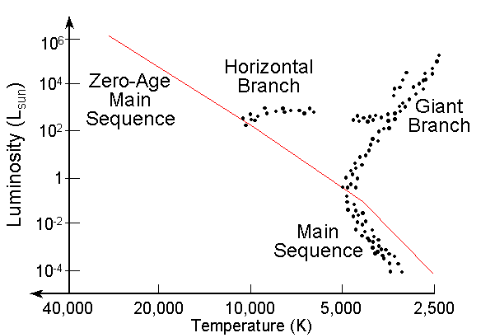
\includegraphics[width=0.309\textwidth]{GA4/Typical Globular Cluster H-R Diagram}
            \caption{Typical Globular Cluster H-R Diagram}
        \end{figure}
        
        \subitem 蓝水平支星(Blue horizontal-branch star, BHB star): 
        \begin{itemize}\small
            \item 核心氦燃烧, 典型质量$0.7M_{\odot}$, $3R_{\odot}$, g波段绝对星等 $\sim$0.7
            \item 颜色偏蓝, 光谱类型V3-A0
            \item 颜色-颜色空间占据狭窄区域, 容易从光度巡天中直接选区样本
        \end{itemize}
        \begin{figure}[!htb]
            \centering
            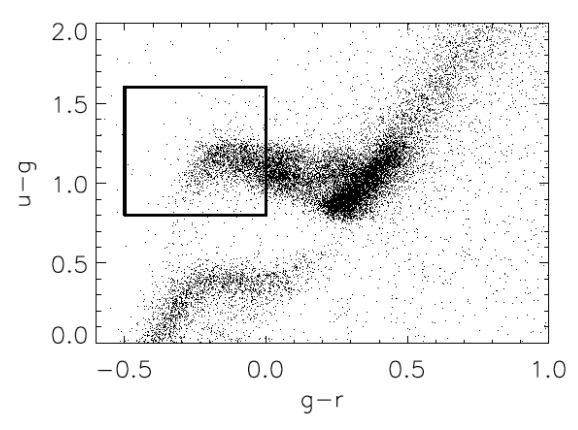
\includegraphics[width=0.309\textwidth]{GA4/颜色-颜色}
            \caption{颜色-颜色}
        \end{figure}
        \subitem K-giant star: 属于贫金属, 红巨星, 由于亮度高, 可以在较远距离出被观测到($\sim$100 Kpc)样本选择更加复杂, 但是一般可以利用其视星等,颜色和金属丰度来得到其绝对星等, 从而计算出距离.   
        \item \textbf{测量示踪恒星的速度分布: }
        \subitem 视向速度可以从光谱中得到(红移/蓝移), 该数据来自光谱巡天, 如SDSS/SEGUE, LAMOST巡天. 
        \subitem 切向速度: 自行测量, 如GAIA. 
        \item \textbf{测量恒星速度弥散度各项异性参数$\beta$: }$\beta$ 的测量并不容易, 除非同时测量到恒星的自行. 在只有视向速度情况下, 一般利用数值模拟给出的$\beta$随半径的分布. 
    \end{enumerate}
    一旦测量了示踪天体的密度、径向速度弥散度、 $\beta$参数 随半径的变化, 可以得到星系的旋转曲线
    \begin{align*}
        -\frac{r}{\rho}\frac{d(\sigma_r^2\rho)}{dr}-2\beta\sigma_r^2=V_{cir}^2(r)
    \end{align*}
    进一步利用银河系的引力势
    \begin{align*}
        \Phi_{tot}(r)=\Phi_{disk}(r)+\Phi_{bulge}(r)+\Phi_{NFW}(r)
    \end{align*}
    分别来自盘, 核球和暗物质晕的引力势. 
    \begin{align*}
        \Phi_{disk}(r)&= -\frac{GM_{disk}(1-e^{-r/b})}{r}\\ 
        \Phi_{bulge}(r)&= -\frac{GM_{bulge}}{r+c_0}\\
        \Phi_{NFW}(r)&=-\frac{4\pi G\rho_s r_{vir}^3}{c^3 r}\ln \left( 1+\frac{cr}{r_{vir}} \right)
    \end{align*}
    代入观测的盘, 核球参数, 利用统计方法(如最小二乘法)拟合旋转曲线, 可得到暗晕质量(其数值一般是延伸到位力半径处). 
\end{enumerate}

如图给出了不同方法测量的银河系暗晕质量. 不同方法给出的结果有差异, 大分布结果集中在 $10^{12}M_{\odot}$ 附近. 
\begin{figure}[!htb]
    \centering
    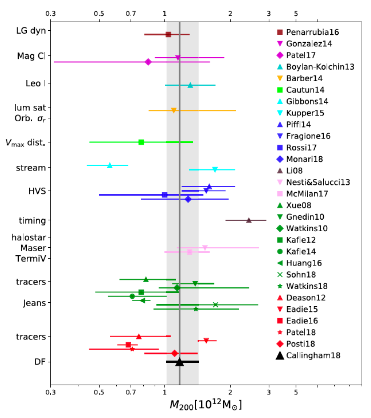
\includegraphics[width=0.309\textwidth]{GA4/暗晕质量}
    \caption{暗晕质量}
\end{figure}

银河系的质量具有非常重要的意义, 它告诉我们: 
\begin{enumerate}
    \item 星系主要是暗物质占主导
    \item 在于其他星系的观测进行比较时, 我们需要限定暗晕质量
\end{enumerate}
